\documentclass{siproblemset}

% SI Session Information
\course{MTH 1321}       % the course of your SI
\sessionnum{idk}         % (optional) specify the session number
\sessiondate{11/30/20}   % the date of the session

\warmup{Concept Review}
\topic{$u$-substitution}
\cooldown{Net change}

% Worksheet Information
\title{Net change and\linebreak $u$-substitution}
\sections{Sections 5.6-5.7}
\withnamespace

\newcommand{\dx}{\text{d}x}

\begin{document}
    \maketitle
    
    \activity{Warmup}{Concept Review}{Work \textbf{alone} to answer these questions. Try not to use your notes.}{15 minutes}
    
    \frq{What is the relationship between the rate of change of a function $r(t)$ and the change in output of the function $\Delta f=f(b)-b(a)$ on the interval $[a,b]$?}
    \Normalsp
    
    \frq{What are the steps to solve a $u$-substitution problem?}
    \newpage
    
    \activity{Activity 1}{FTOCII and Graphs}{Make a \textbf{group of two or three, all with the differently-colored worksheets}, to work together to answer these questions. Try not to use your notes. \textbf{DO NOT use a calculator}.}{30 minutes}
    
    \begin{multipartquestion}
        Let $A(x)=\int_0^xf(t)\text{d}t$. Use the graph of $f(x)$ below to answer the following questions. 
        \makebox[\width][c]{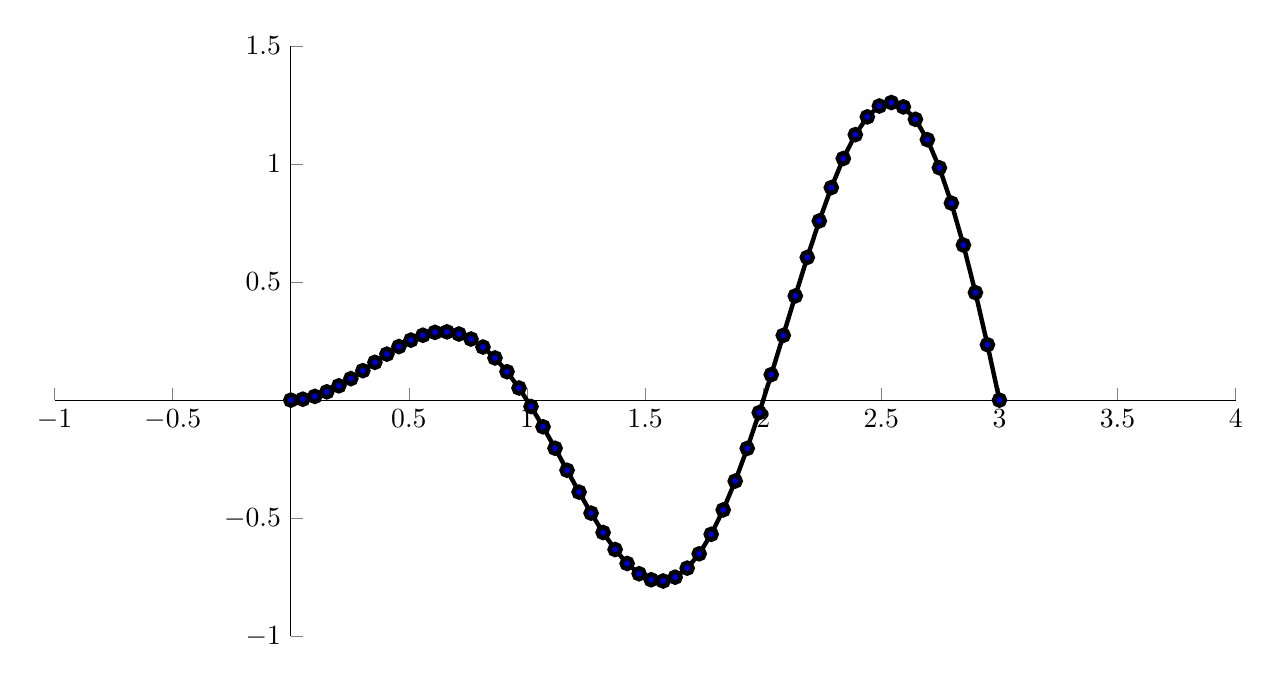
\begin{tikzpicture}[baseline=(current bounding box.north)]
            \begin{axis}[
            x=3cm,
            y=3cm,
            xmin=-1,
            xmax=4,
            ymin=-1,
            ymax=1.5,
            axis x line*=middle,
            axis y line*=middle,
            every axis plot/.append style={ultra thick},
            samples=60
            ]
            \addplot+[black, domain=0:3] {sin(180*x)*x/2};
            \end{axis}
            \end{tikzpicture}} 
        
        \frq{What are the intervals of increase and decrease for $A$?}
        \smallsp
        \frq{What are the $x$-values where $A$ has a local extremum?}
        \smallsp
        \frq{Where is $A$ concave up and down?}
        \smallsp
    \end{multipartquestion}
    
    \newpage
    
    \frq{Find the \textbf{total} area between the graph of $f(x)=x^2-1$ and the $x$-axis, only considering the region satisfying $-3\leq x\leq 3$.}
    \Hugesp
    
    \activity{Activity 2}{Net change}{Make a \textbf{group of two or three, all with the same colored worksheets}, to work together to do your assigned parts. Then, try to do the other parts. Try not to use your notes. \textbf{DO NOT use a calculator}.}{30 minutes}
    
    \frq{A survey shoes that a candidate is gaining votes at a rate of $2000t+1000$ votes per day, where $t$ is the number of days since she announced her candidacy. How many supporters will the candidate have after 60 days (assuming that she had no supporters at $t=0$)?}
    \largespace
    
    \frq{A particle moves in a straight line with velocity $v(t)=t^{-2}-1$ m/s. Find the displacement and total distance traveled over the time interval $[0.5,2]$ seconds.}
    \hugespace
    
    \frq{Over the course of $\pi$ seconds, a particle moves in a straight line with velocity $v(t)=t+\sin t$ m/s. What was the total distance and displacement of the particle on its journey?}
    \hugespace
    
    \frq{Water flows out of a $10000$L tank at a rate of $1000+25t$ liters per hour (where $t$ is in hours). Assuming the tank was full to start, how much water is left after $4$ hours?}
    \hugespace
    
    \frq{The traffic flow rate past a certain point on a highway is $q(t)=3000+2000t-300t^2$ ($t$ is in hours), where $t=0$ is 8am. How many cars pass by in the time interval from 8 to 10am?}
    \largespace
    \newpage
    
    \activity{Cooldown}{Basic $u$-substitution}{Make a \textbf{group of two or three, all with the same colored worksheets}, to work together to do your assigned parts. Then, try to do the other parts. Try not to use your notes. \textbf{DO NOT use a calculator}.}{30 minutes}
        
    \mcq{Compute the following indefinite integrals.}{
        \task $\int\frac{\dx}{\sqrt{x}\paren{1+\sqrt{x}}^2}$
        \Smallsp
        \task $\int\sec^2(\theta)\tan(\theta)\dd\theta$
        \Smallsp
        \task $\int\sqrt{4x-1}\dx$
        \Smallsp
        \task $\int t\sqrt{4t-1}\dd t$
        \Smallsp
        \task $\int \dfrac{x+1}{\sqrt{x+1}}\dd x$
    }
%    \newpage
%
%    \activity{Activity 2}{Bounded $u$-substitution}{Make a \textbf{group of two or three, all with the same colored worksheets}, to work together to do your assigned parts. Then, try to do the other parts. Try not to use your notes. \textbf{DO NOT use a calculator}.}{30 minutes}
%    \mcq{Compute the following definite integrals.}{
%        \task $\int_{-8/3}^{-2}(3x+8)^{11}\dx$
%        \Smallsp
%        \task $\int_{1}^{2}\frac{t\dd t}{\sqrt{t^2+9}}$
%        \Smallsp
%        \task $\int_{\arcsin{(\pi/4)}}^{\arcsin{(\pi/2)}}\cos(\theta)\cos(\sin(\theta))\dd\theta$
%        \Smallsp
%        \task $\int_{1}^{2}xe^{x^2}\dx$
%        \Smallsp
%    }
%\newpage
%    \activity{Cooldown}{Net change}{Make a \textbf{group of two or three, all with the same colored worksheets}, to work together to do your assigned parts. Then, try to do the other parts. Try not to use your notes. \textbf{DO NOT use a calculator}.}{30 minutes}
%    
%      \frq{A survey shoes that a candidate is gaining votes at a rate of $2000t+1000$ votes per day, where $t$ is the number of days since she announced her candidacy. How many supporters will the candidate have after 60 days (assuming that she had no supporters at $t=0$)?}
%    \largespace
%    
%    \frq{A particle moves in a straight line with velocity $v(t)=t^{-2}-1$ m/s. Find the displacement and total distance traveled over the time interval $[0.5,2]$ seconds.}
%    \hugespace
%    
%    \frq{Over the course of $\pi$ seconds, a particle moves in a straight line with velocity $v(t)=t+\sin t$ m/s. What was the total distance and displacement of the particle on its journey?}
%    \hugespace
%    
%    \frq{Water flows out of a $10000$L tank at a rate of $1000+25t$ liters per hour (where $t$ is in hours). Assuming the tank was full to start, how much water is left after $4$ hours?}
%    \pagebreak
%    
%    \frq{The traffic flow rate past a certain point on a highway is $q(t)=3000+2000t-300t^2$ ($t$ is in hours), where $t=0$ is 8am. How many cars pass by in the time interval from 8 to 10am?}
%    \largespace
%\newpage
%    \activity{Bonus}{Harder $u$-substitution}{Make a \textbf{group of two or three, all with the same colored worksheets}, to work together to do your assigned parts. Then, try to do the other parts. Try not to use your notes. \textbf{DO NOT use a calculator}.}{30 minutes}
%    
%    \mcq{Compute the following integrals.}{
%        \task $\int\dfrac{x+\ln x}{x}\dd x$
%        \Normalsp
%        \task $\int\cot x\dd x$
%        \Smallsp
%        \task $\int_{-3}^{1}2xe^{x^2+3x}+3e^{x^2+3x}\dx$
%    }
\end{document}